\documentclass[11pt,a4paper]{article}
\usepackage[margin=2.2cm]{geometry}
\usepackage{graphicx}
\usepackage{booktabs}
\usepackage{caption}
\usepackage{float}
\usepackage{amsmath}
\usepackage[hidelinks]{hyperref}
\captionsetup{font=small,labelfont=bf}
% generated by scripts/make_results_report.py -- do not edit
\newcommand{\inlaGainA}{5.3}
\newcommand{\jsdBaseA}{0.1190}
\newcommand{\jsdInlaA}{0.1126}
\newcommand{\jsdStateA}{0.0971}
\newcommand{\jsdTrendsA}{0.1039}
\newcommand{\jsdWeatherA}{0.1175}
\newcommand{\nRows}{3{,}194}
\newcommand{\nRowsC}{3{,}723}
\newcommand{\onsetBase}{2.99}
\newcommand{\onsetState}{2.44}
\newcommand{\onsetTrends}{2.57}
\newcommand{\peakBase}{6.41}
\newcommand{\peakState}{5.43}
\newcommand{\peakTrends}{5.77}
\newcommand{\peakWithinTwoBase}{29}
\newcommand{\peakWithinTwoState}{41}
\newcommand{\peakWithinTwoTrends}{38}
\newcommand{\statesTotal}{27}
\newcommand{\statesWorse}{4}
\newcommand{\statesWorseList}{PI, AP, AC, RR}
\newcommand{\trendsCImuniA}{[-13.9, -11.6]}
\newcommand{\trendsCIyearA}{[-17.9, -8.4]}
\newcommand{\trendsGainA}{12.7}
\newcommand{\trendsGainC}{12.8}
\newcommand{\trendsShareBetter}{72}
\newcommand{\trendsVsInla}{7.8}
\newcommand{\trendsYearsA}{12 of 12}
\newcommand{\trendsYearsC}{14 of 14}
\newcommand{\weatherGainA}{1.3}
\newcommand{\weatherOnTrendsA}{+1.7}
\newcommand{\weatherOnTrendsYearsA}{4 of 12}
\newcommand{\wyTest}{0.1320}
\newcommand{\wyTwo}{0.1185}


\title{Rebuilding Weekly Dengue Curves from Annual Totals:\\Results, Ablation Study and Discussion}
\author{Aminah\\FAST-NUCES Islamabad}
\date{November 2026}

\begin{document}
\maketitle

\begin{abstract}
We rebuild the weekly dengue curve of a municipality from its known annual total and ask which information improves the
rebuilt shape. On 300 Brazilian municipalities (2010--2023, \nRows{} held-out municipality-years in the main design),
local weather lowers the shape error by only \weatherGainA\,\% relative to a seasonal Dirichlet-multinomial baseline
(B4s), and the base paper's scaled INLA by \inlaGainA\,\%. Adding same-year Google Trends search interest lowers it by
\trendsGainA\,\% (95\,\% year-bootstrap interval \trendsCIyearA\,\%), better in \trendsYearsA{} test years, and the gain
replicates in a second validation design (\trendsGainC\,\%, \trendsYearsC{} years) and at every training length
from two to thirteen years (\lcGainMin--\lcGainMax\,\% with $k=2$--9 training years). Ablations show that the gain comes
from the timing of the right year (it disappears with another year's searches), that weather adds nothing once search
data are included, and that the gain is smallest in the North and in states with few searches. All numbers, tables and
figures in this document are generated by one script from the committed run outputs (Section~\ref{sec:repro}).
\end{abstract}

\section{Problem and research gaps}
Many dengue records are annual, while planning, forecasting and climate--health studies need weekly curves. The base
paper (Lim et al., 2026) splits annual totals into sub-annual shares with a Dirichlet-multinomial (DM) model and selects
scaled INLA as its final method; in both, every rebuilt year of a place receives essentially the same seasonal shape,
so epidemics that start early or late are missed. Related work either validates against synthetic or single-year data
(Morello et al., 2026; Al Mobin et al., 2023, 2025), adds only climate (Rozo Posada et al., 2026), or uses search data
for nowcasting rather than for rebuilding past years (Yang et al., 2017; Xiao et al., 2025). This document reports the
experiments that address these gaps:
(G1) a year-specific shape instead of one fixed shape;
(G2) validation against true weekly counts over many years;
(G3) a head-to-head comparison of climate with a same-year search signal; and
(G4) component-level evidence of where the gain comes from.

\section{Experimental setup}
\paragraph{Data.} Weekly notified dengue cases (InfoDengue) for 300 municipalities in all 27 states, 2010--2023; NASA
POWER weather (CHIRPS rain as a check); the Oceanic Ni\~no Index (ONI); weekly Google Trends interest for ``dengue'' for
Brazil and each state (five overlapping four-year windows, 140 files, kept as a snapshot). The year 2024 is locked and
never loaded.
\paragraph{Task and metric.} The annual total $N$ of a held-out municipality-year is known; a model predicts the share of
$N$ in each epidemiological week, and the counts are allocated to sum exactly to $N$. The primary metric is the
Jensen--Shannon divergence (JSD) between the true and rebuilt weekly shares (0 = identical; multinomial noise floor
$\approx 0.015$). Secondary metrics: peak-week error and onset-week error (week in which 10\,\% of the cases are
reached), in weeks. ``Change \%'' is the relative change in mean JSD; negative means less error.
\paragraph{Validation designs.} Design A (primary): expanding window, train on 2010 to $T-1$, test $T=2012,\dots,2023$
(12 folds). Design C: leave one year out (14 folds, \nRowsC{} rows). Design B: fixed test years (2019, 2021, 2023) with
$k$ preceding training years (learning curve). All models share folds, municipalities and evaluation rows.
\paragraph{Models.} B0 (uniform), B1 (seasonal profile), B4 (base paper's DM), B4s (B4 + annual-size terms; the
comparator), M1/M1-noONI/M1-short (B4s + weather anomalies at lags 0--20 weeks, with/without ONI, or lags 0--3 only),
M2 (boosted softmax with weather), scaled INLA (base paper's final model, $\pm$ weather). Timing models add same-year
signals to B4s: S2 (Google Trends anomalies, lags 0--3), S2C (S2 + weather), T1 (seasonal shape shifted by the
estimated timing shift), and, as an upper bound only, S1 (curve of the other towns of the same state in the same year,
target left out), S3 (S1 + S2) and S3C (S3 + weather). S1/S3 need same-year weekly counts of neighbours, which a truly
missing year does not have.
\paragraph{Statistics.} Paired bootstraps (2{,}000 replicates, seed 1) resampling municipalities or test years; a
difference is called clear only if both intervals exclude zero.

\section{Results}
\begin{table}[t]
\centering
\small
\caption{Mean shape error (JSD, lower is better) of every model on design A (expanding window, 12 test years, 3{,}194 municipality-years) and design C (leave one year out, 14 folds). Negative ``vs B4s'' = less error than the B4s baseline. Scaled INLA was run on design A only.}
\label{tab:main}
\resizebox{\linewidth}{!}{%
\begin{tabular}{llrrrrrrr}
\toprule
Model & Description & JSD (A) & 95\% CI (towns) & vs B4s \% & Peak err (wk) & Onset err (wk) & JSD (C) & vs B4s \% (C) \\
\midrule
B0 & Uniform weeks & 0.1861 & [0.1797, 0.1926] & +56.4 & 11.74 & -- & 0.1888 & +70.0 \\
B1 & Seasonal profile & 0.1282 & [0.1230, 0.1337] & +7.7 & 6.27 & 3.22 & 0.1197 & +7.8 \\
B4 & Base paper's DM & 0.1256 & [0.1204, 0.1310] & +5.6 & 6.22 & -- & 0.1191 & +7.2 \\
B4s & DM + annual size (baseline) & 0.1190 & [0.1137, 0.1247] & -- & 6.41 & 2.99 & 0.1110 & -- \\
\midrule
M1-noONI & B4s + local weather & 0.1175 & [0.1121, 0.1232] & -1.3 & 6.25 & 2.91 & 0.1077 & -3.0 \\
M1 & B4s + weather + ONI & 0.1191 & [0.1138, 0.1247] & +0.1 & 6.26 & 2.90 & 0.1090 & -1.8 \\
M1-short & B4s + weather, lags 0--3 wk & 0.1166 & [0.1114, 0.1223] & -2.0 & 6.30 & -- & 0.1089 & -1.9 \\
M2 & Boosted softmax (weather) & 0.1267 & [0.1216, 0.1321] & +6.5 & 6.21 & -- & 0.1182 & +6.4 \\
\midrule
INLA-scaled & Scaled INLA (base paper's final) & 0.1126 & [0.1084, 0.1171] & -5.3 & 5.74 & -- & -- & -- \\
INLA-scaled-clim15 & Scaled INLA + local weather & 0.1110 & [0.1068, 0.1154] & -6.7 & 5.68 & -- & -- & -- \\
INLA-scaled-clim20 & Scaled INLA + weather + ONI & 0.1131 & [0.1088, 0.1175] & -4.9 & 5.70 & -- & -- & -- \\
\midrule
T1 & B4s, seasonal shape shifted & 0.1096 & [0.1039, 0.1155] & -7.9 & 5.70 & 2.55 & 0.1041 & -6.2 \\
S2 & B4s + Google Trends & 0.1039 & [0.0985, 0.1096] & -12.7 & 5.77 & 2.57 & 0.0968 & -12.8 \\
S2C-noONI & S2 + local weather & 0.1056 & [0.1003, 0.1113] & -11.2 & 5.80 & 2.58 & 0.0968 & -12.8 \\
S2C & S2 + weather + ONI & 0.1073 & [0.1019, 0.1129] & -9.9 & 5.84 & 2.60 & 0.0979 & -11.8 \\
\midrule
S1 & B4s + state curve (upper bound) & 0.0971 & [0.0920, 0.1026] & -18.4 & 5.43 & 2.44 & 0.0871 & -21.6 \\
S3 & S1 + Google Trends (upper bound) & 0.0963 & [0.0912, 0.1018] & -19.1 & 5.41 & 2.41 & 0.0868 & -21.8 \\
S3C & S3 + weather + ONI (upper bound) & 0.0991 & [0.0940, 0.1046] & -16.7 & 5.45 & 2.44 & 0.0873 & -21.4 \\
\bottomrule
\end{tabular}}
\par\vspace{2pt}\footnotesize Upper-bound rows need the same year's weekly counts of other towns in the state, which a truly missing year does not have; they are reported as a ceiling, not as a usable method.
\end{table}


Table~\ref{tab:main} and Figure~\ref{fig:models} compare all models. Weather moves the error by about 1\,\%; scaled INLA
reaches \jsdInlaA{} (\inlaGainA\,\% below B4s); the search model S2 reaches \jsdTrendsA{}, \trendsGainA\,\% below B4s
and \trendsVsInla\,\% below scaled INLA. Only the state-curve upper bound is lower (\jsdStateA).

\begin{figure}[t]
\centering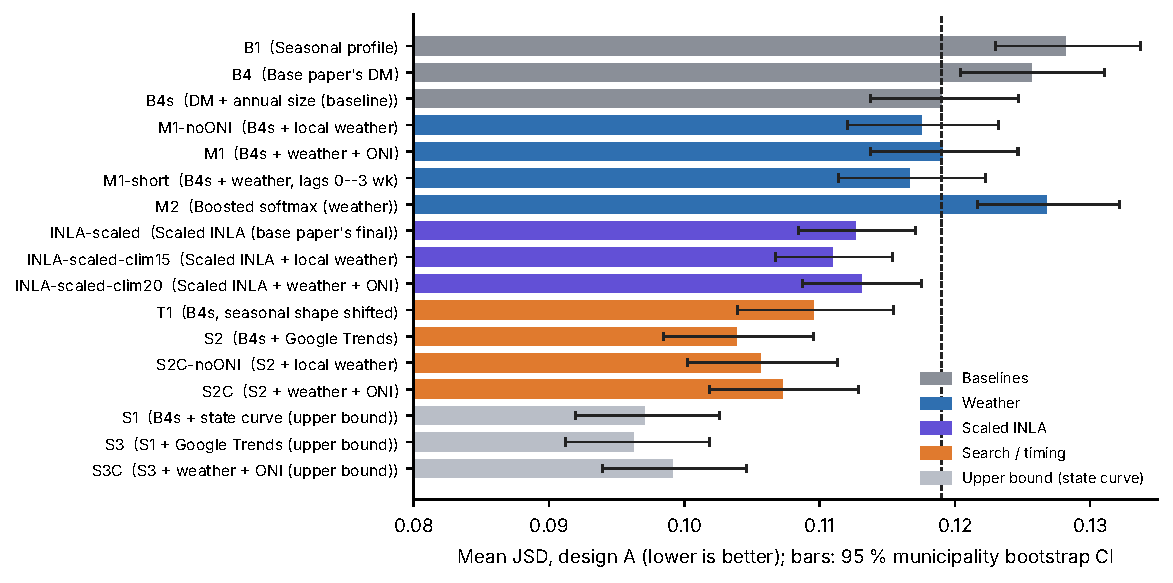
\includegraphics[width=0.92\linewidth]{figures/fig1_model_comparison.pdf}
\caption{Mean JSD of every model in design A with 95\,\% municipality bootstrap intervals; dashed line: B4s.}
\label{fig:models}
\end{figure}

\begin{table}[t]
\centering
\small
\caption{Paired bootstrap tests (2{,}000 replicates) of the main contrasts in both designs. \% = relative change in mean JSD of the first model vs the second; ``years'' = test years in which the first model had the lower mean JSD.}
\label{tab:contrasts}
\resizebox{\linewidth}{!}{%
\begin{tabular}{lrrrrrrrr}
\toprule
Contrast & A: \% & A: CI towns & A: CI years & A: years & C: \% & C: CI towns & C: CI years & C: years \\
\midrule
S2 vs B4s & -12.7 & [-13.9, -11.6] & [-17.9, -8.4] & 12/12 & -12.8 & [-14.2, -11.4] & [-18.8, -7.5] & 14/14 \\
S2 vs M1-noONI & -11.6 & [-12.6, -10.6] & [-15.3, -8.5] & 12/12 & -10.1 & [-11.4, -8.9] & [-15.4, -5.0] & 12/14 \\
S2C-noONI vs S2 & +1.7 & [+1.2, +2.2] & [-0.8, +4.3] & 4/12 & +0.1 & [-0.3, +0.4] & [-1.0, +1.2] & 6/14 \\
T1 vs B4s & -7.9 & [-9.4, -6.4] & [-13.3, -3.0] & 11/12 & -6.2 & [-7.5, -4.9] & [-10.8, -2.0] & 12/14 \\
S1 vs B4s & -18.4 & [-19.8, -17.0] & [-24.2, -13.5] & 12/12 & -21.6 & [-23.1, -20.0] & [-28.3, -14.9] & 14/14 \\
S3 vs S1 & -0.8 & [-1.1, -0.6] & [-1.4, -0.5] & 11/12 & -0.3 & [-0.6, +0.0] & [-1.2, +0.8] & 11/14 \\
\bottomrule
\end{tabular}}
\end{table}


\paragraph{Is the search gain significant?} Table~\ref{tab:contrasts} gives the paired tests. S2 is better than B4s
with both intervals well below zero in both designs (design A: \trendsGainA\,\% less error, municipality interval
\trendsCImuniA\,\%, year interval \trendsCIyearA\,\%; better in \trendsYearsA{} years; design C: \trendsYearsC{}).
It is also clearly better than the weather model M1-noONI. At the level of single municipality-years, S2 has the lower
error in \trendsShareBetter\,\% of the \nRows{} cases (Figure~\ref{fig:dist}, left).

\begin{figure}[t]
\centering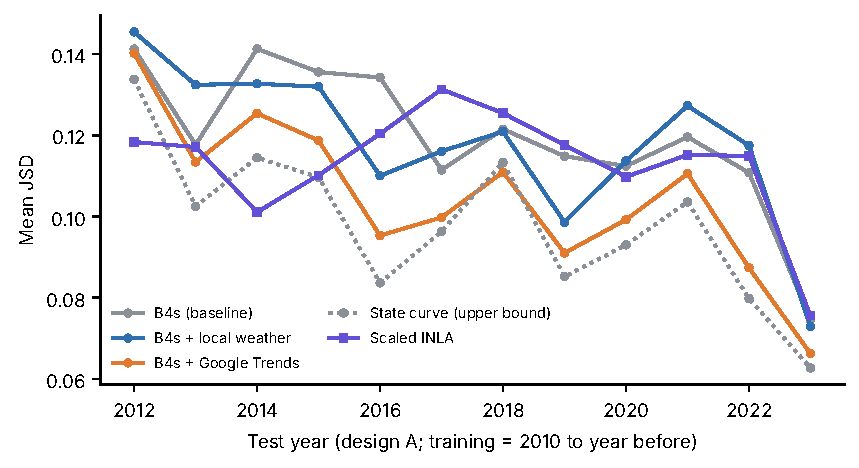
\includegraphics[width=0.92\linewidth]{figures/fig2_jsd_by_year.pdf}
\caption{Mean JSD by test year in design A. The training window grows with the test year.}
\label{fig:years}
\end{figure}

\begin{figure}[t]
\centering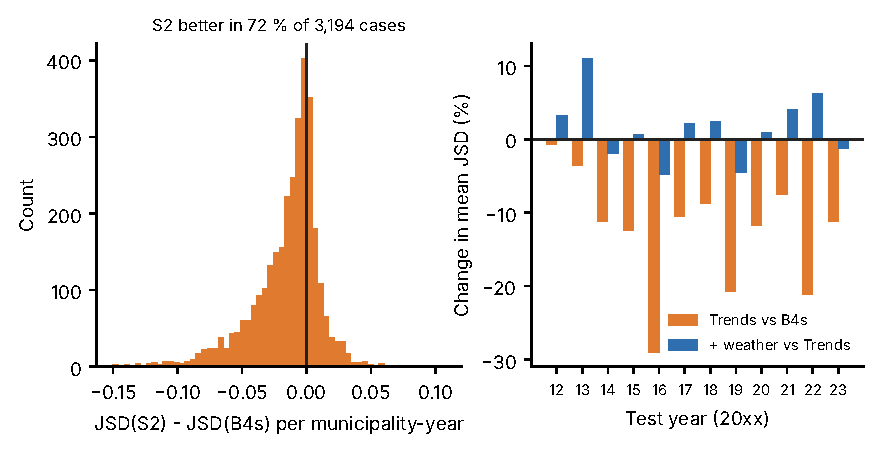
\includegraphics[width=0.95\linewidth]{figures/fig3_gain_distribution.pdf}
\caption{Left: distribution of the paired difference JSD(S2) $-$ JSD(B4s) over municipality-years (values clipped
at $\pm0.15$). Right: change in mean JSD per test year for Trends vs B4s and for adding weather to Trends.}
\label{fig:dist}
\end{figure}

\paragraph{Timing.} Figure~\ref{fig:years} shows that the search model is below the baseline and the weather model in
every test year. In practical units (Figure~\ref{fig:ecdf}), the mean peak-week error falls from \peakBase{} (B4s) to
\peakTrends{} weeks (S2) and the onset error from \onsetBase{} to \onsetTrends{} weeks; the share of municipality-years
whose peak is placed within two weeks rises from \peakWithinTwoBase\,\% to \peakWithinTwoTrends\,\%.

\begin{figure}[t]
\centering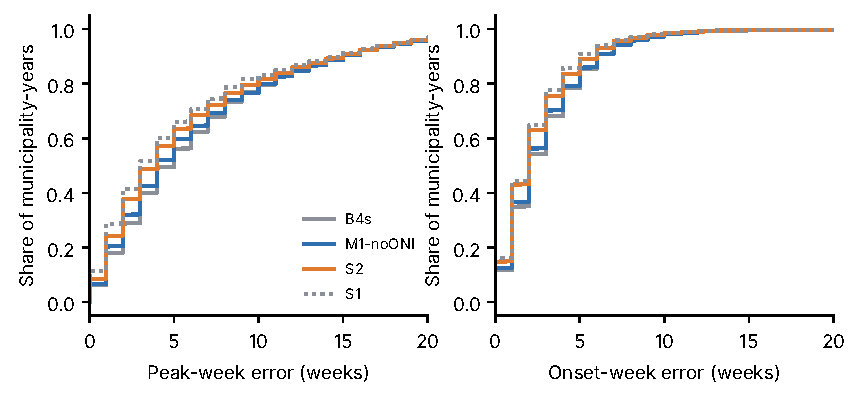
\includegraphics[width=0.92\linewidth]{figures/fig5_peak_onset_ecdf.pdf}
\caption{Cumulative distribution of peak-week (left) and onset-week (right) errors, design A. Curves further up and
left are better.}
\label{fig:ecdf}
\end{figure}

\paragraph{Training length.} The learning curve of the climate study (design B, Figure~\ref{fig:lc}) shows that all
models improve once each municipality has at least three training years, and that the weather model needs about five
years before it stops hurting. With two years every model falls back on regional profiles, so $k=2$ is out of line.

We ran the same learning curve with the search models, from one training year (train 2010, test 2011) to thirteen
(Table~\ref{tab:lc}, Figure~\ref{fig:lctrends}). Google Trends lowers the error at every training length from two
years on: by \lcGainTwo\,\% with only two training years and by \lcGainMin--\lcGainMax\,\% for $k=2$--9, with all
municipality intervals below zero. Weather, in contrast, is harmful with two training years (\lcWeatherTwo\,\%) and
helps by about 3\,\% from $k \ge 4$; adding weather to Trends is harmful with few years (\lcWeatherOnTrendsTwo\,\% at
$k=2$) and neutral from $k \ge 6$. With a single training year the search model reduces exactly to B4s: its features
are anomalies relative to the training years, which are all zero when there is only one training year, so nothing
can be learned. The search signal therefore needs at least two years of history, but not more, which matters for
countries with short weekly records.

\begin{table}[t]
\centering
\small
\caption{Learning curve with Google Trends. $k$ = number of training years immediately before the test year. $k=1$: train 2010, test 2011. $k=2$--9: all three fixed test years (2019, 2021, 2023); $k \ge 10$: fewer test years remain, so these rows are not comparable with the others.}
\label{tab:lc}
\resizebox{\linewidth}{!}{%
\begin{tabular}{llrrrrrr}
\toprule
k & Test years & B4s & S2 (Trends) & Trends vs B4s \% & 95\% CI towns & Weather vs B4s \% & Weather on Trends \% \\
\midrule
1 & 2011 & 0.1014 & 0.1014 & +0.0 & [+0.0, +0.0] & +7.2 & +7.2 \\
\midrule
2 & 2019 2021 2023 & 0.1056 & 0.0929 & -12.0 & [-14.1, -10.0] & +11.3 & +9.8 \\
3 & 2019 2021 2023 & 0.1424 & 0.1101 & -22.7 & [-25.0, -20.3] & -1.5 & +3.0 \\
4 & 2019 2021 2023 & 0.1184 & 0.0986 & -16.8 & [-18.9, -14.7] & -2.9 & +1.0 \\
5 & 2019 2021 2023 & 0.1112 & 0.0932 & -16.2 & [-18.4, -13.9] & -2.8 & +1.1 \\
6 & 2019 2021 2023 & 0.1095 & 0.0915 & -16.4 & [-18.6, -14.3] & -3.2 & +0.3 \\
7 & 2019 2021 2023 & 0.1071 & 0.0896 & -16.3 & [-18.5, -14.2] & -3.9 & +0.3 \\
8 & 2019 2021 2023 & 0.1045 & 0.0881 & -15.8 & [-17.8, -13.7] & -3.4 & +0.0 \\
9 & 2019 2021 2023 & 0.1027 & 0.0881 & -14.1 & [-16.0, -12.3] & -3.4 & -0.8 \\
\midrule
10 & 2021 2023 & 0.0959 & 0.0863 & -10.0 & [-12.2, -7.7] & +3.4 & +1.3 \\
11 & 2021 2023 & 0.0954 & 0.0863 & -9.5 & [-11.5, -7.4] & +3.4 & +2.4 \\
12 & 2023 & 0.0743 & 0.0658 & -11.5 & [-14.4, -8.5] & -1.1 & -0.4 \\
13 & 2023 & 0.0746 & 0.0663 & -11.2 & [-13.9, -8.4] & -2.2 & -1.3 \\
\bottomrule
\end{tabular}}
\par\vspace{2pt}\footnotesize Year-bootstrap intervals are not given: at most three test years per row.
\end{table}


\begin{figure}[t]
\centering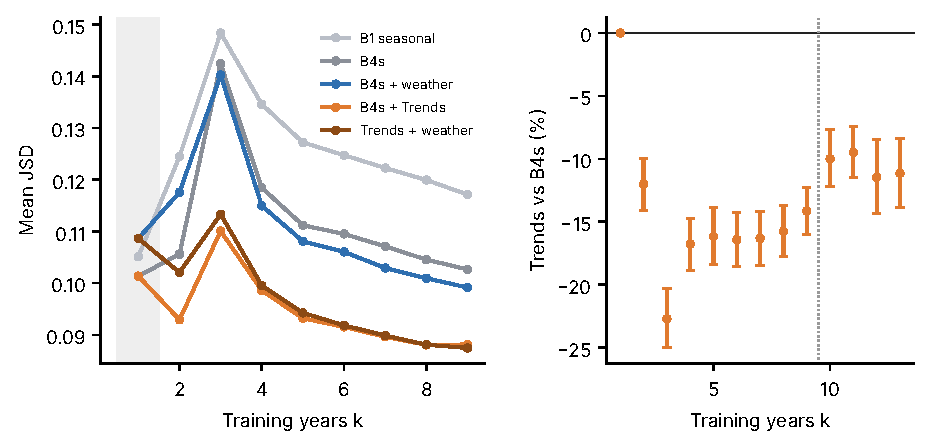
\includegraphics[width=0.95\linewidth]{figures/fig10_learning_curve_trends.pdf}
\caption{Learning curve with Google Trends. Left: mean JSD by number of training years $k$ (grey band: $k=1$, test
year 2011). Right: change in mean JSD of B4s + Trends vs B4s with 95\,\% municipality bootstrap intervals; right of the
dotted line fewer test years remain.}
\label{fig:lctrends}
\end{figure}

\begin{figure}[t]
\centering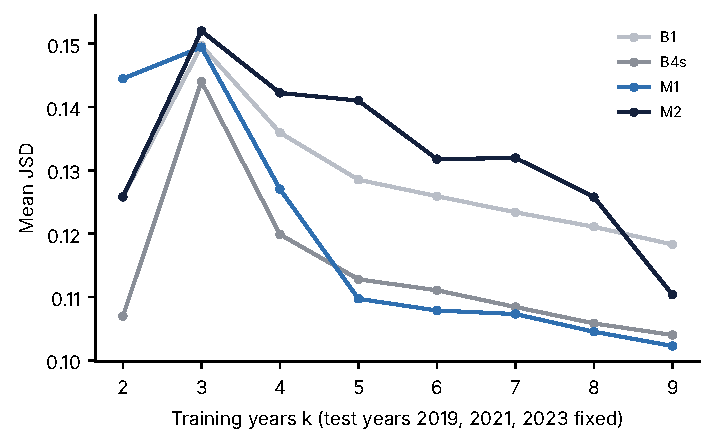
\includegraphics[width=0.62\linewidth]{figures/fig6_learning_curve.pdf}
\caption{Learning curve (design B): mean JSD against the number of training years, averaged over the three fixed test
years. From the official climate run.}
\label{fig:lc}
\end{figure}

\begin{table}[t]
\centering
\small
\caption{Automatic checks of the timing-model runs, from the run check files.}
\label{tab:audits}
\resizebox{\linewidth}{!}{%
\begin{tabular}{lrlll}
\toprule
Design & Folds & Leakage audit & Feature audit (train-only) & Exact sums \\
\midrule
A & 12 & pass & pass & pass \\
C & 14 & pass & pass & pass \\
\bottomrule
\end{tabular}}
\end{table}

\paragraph{Integrity checks.} Every fold passed the leakage audit and the feature audit, which recomputes the search and
state-curve climatologies after replacing all non-training years with random numbers (Table~\ref{tab:audits}).

\section{Ablation study}
\begin{table}[t]
\centering
\small
\caption{Ablation study, design A: each row adds, removes or alters one component and reports the paired change in mean JSD (negative = the component lowers the error). ``Clearly'' requires both the municipality and the year bootstrap intervals to exclude zero.}
\label{tab:ablation}
\resizebox{\linewidth}{!}{%
\begin{tabular}{llrrrrrrl}
\toprule
Component changed & Models & JSD with & JSD without & Change \% & 95\% CI towns & 95\% CI years & Years better & Verdict \\
\midrule
Annual size terms & B4s vs B4 & 0.1190 & 0.1256 & -5.3 & [-6.6, -4.0] & [-10.1, +0.9] & 10/12 & not clear \\
Local weather & M1-noONI vs B4s & 0.1175 & 0.1190 & -1.3 & [-2.0, -0.6] & [-6.6, +3.7] & 6/12 & not clear \\
ONI on top of local weather & M1 vs M1-noONI & 0.1191 & 0.1175 & +1.4 & [+0.8, +1.9] & [-0.8, +4.6] & 5/12 & not clear \\
Long lags (0--20 vs 0--3 wk) & M1 vs M1-short & 0.1191 & 0.1166 & +2.1 & [+1.6, +2.6] & [-1.5, +5.8] & 3/12 & not clear \\
Boosted learner instead of DM & M2 vs B4s & 0.1267 & 0.1190 & +6.5 & [+5.2, +7.8] & [-0.5, +12.5] & 2/12 & not clear \\
\midrule
Scaled INLA instead of B4s & INLA-scaled vs B4s & 0.1126 & 0.1190 & -5.3 & -- & [-11.7, +1.4] & 7/12 & not clear \\
\midrule
Shift-only timing (T1) & T1 vs B4s & 0.1096 & 0.1190 & -7.9 & [-9.4, -6.4] & [-13.3, -3.0] & 11/12 & clearly better \\
Google Trends block (S2) & S2 vs B4s & 0.1039 & 0.1190 & -12.7 & [-13.9, -11.6] & [-17.9, -8.4] & 12/12 & clearly better \\
Local weather on top of Trends & S2C-noONI vs S2 & 0.1056 & 0.1039 & +1.7 & [+1.2, +2.2] & [-0.8, +4.3] & 4/12 & not clear \\
ONI on top of Trends + weather & S2C vs S2C-noONI & 0.1073 & 0.1056 & +1.6 & [+1.1, +2.0] & [+0.2, +4.0] & 2/12 & clearly worse \\
\midrule
State-curve block (S1) & S1 vs B4s & 0.0971 & 0.1190 & -18.4 & [-19.8, -17.0] & [-24.2, -13.5] & 12/12 & clearly better \\
Trends on top of state curve & S3 vs S1 & 0.0963 & 0.0971 & -0.8 & [-1.1, -0.6] & [-1.4, -0.5] & 11/12 & clearly better \\
Weather + ONI on top of S3 & S3C vs S3 & 0.0991 & 0.0963 & +2.9 & [+2.4, +3.5] & [+1.4, +4.4] & 3/12 & clearly worse \\
State curve as features vs shift & S1 vs T1 & 0.0971 & 0.1096 & -11.4 & [-12.6, -10.2] & [-14.4, -8.2] & 12/12 & clearly better \\
\midrule
State curve from 50 \% of towns & S1-p50 vs S1 & 0.0984 & 0.0971 & +1.4 & [+0.9, +2.0] & [+0.8, +2.0] & 1/12 & clearly worse \\
State curve from 25 \% of towns & S1-p25 vs S1 & 0.0996 & 0.0971 & +2.6 & [+1.8, +3.3] & [+1.5, +3.9] & 1/12 & clearly worse \\
State curve, non-study towns only & S1-ns vs S1 & 0.1026 & 0.0971 & +5.7 & [+4.3, +7.1] & [+3.9, +7.8] & 0/12 & clearly worse \\
\midrule
Wrong-year Trends (refitted) & S2-wy vs S2 & 0.1185 & 0.1039 & +14.1 & [+12.8, +15.7] & [+8.7, +21.2] & 1/12 & clearly worse \\
Wrong-year state curve (refitted) & S1-wy vs S1 & 0.1185 & 0.0971 & +22.1 & [+20.1, +24.2] & [+15.1, +31.4] & 0/12 & clearly worse \\
Wrong-year signals at test only & S3-wyTest vs S3 & 0.1320 & 0.0963 & +37.2 & [+34.0, +40.5] & [+26.9, +49.9] & 0/12 & clearly worse \\
\bottomrule
\end{tabular}}
\par\vspace{2pt}\footnotesize Scaled INLA: per-municipality rows are not stored, so only the year-level interval is given. Rows 1, 4 and 5 come from the official climate run (same folds and municipalities).
\end{table}


Table~\ref{tab:ablation} and Figure~\ref{fig:ablation} isolate one component per row (design A, paired).
\begin{itemize}
\item \textbf{Annual size} (B4s vs B4) is the most useful element of the baseline; \textbf{weather} gives a small
municipality-level gain that is not clear across years; \textbf{ONI} and \textbf{long lags} make it worse; a
\textbf{flexible learner} (M2) is worse than the DM.
\item \textbf{Same-year timing} is the decisive component: even a pure shift of the seasonal shape (T1) is clearly
better than B4s, and the search block (S2) roughly doubles that gain.
\item \textbf{Weather on top of search} does not help (\weatherOnTrendsA\,\%, better in only \weatherOnTrendsYearsA{}
years); adding ONI on top is clearly worse. Search on top of the state curve adds less than 1\,\%.
\item \textbf{Features vs shift:} entering the state curve as anomaly features (S1) is clearly better than shifting the
seasonal shape (T1), so the signal carries more than a single timing offset.
\item \textbf{Fewer reporting towns:} a state curve from a random 50\,\% or 25\,\% of towns keeps most of the gain; from
non-study towns only it still beats B4s by a wide margin.
\item \textbf{Wrong-year controls:} refitting with another year's searches or state curve removes the gain (S2-wy:
\wyTwo, the level of B4s; Figure~\ref{fig:wy}); feeding another year's signals at test time only makes the model worse
than the seasonal baseline (\wyTest). The gain therefore comes from the right year's timing, not from model capacity.
\end{itemize}

\begin{figure}[t]
\centering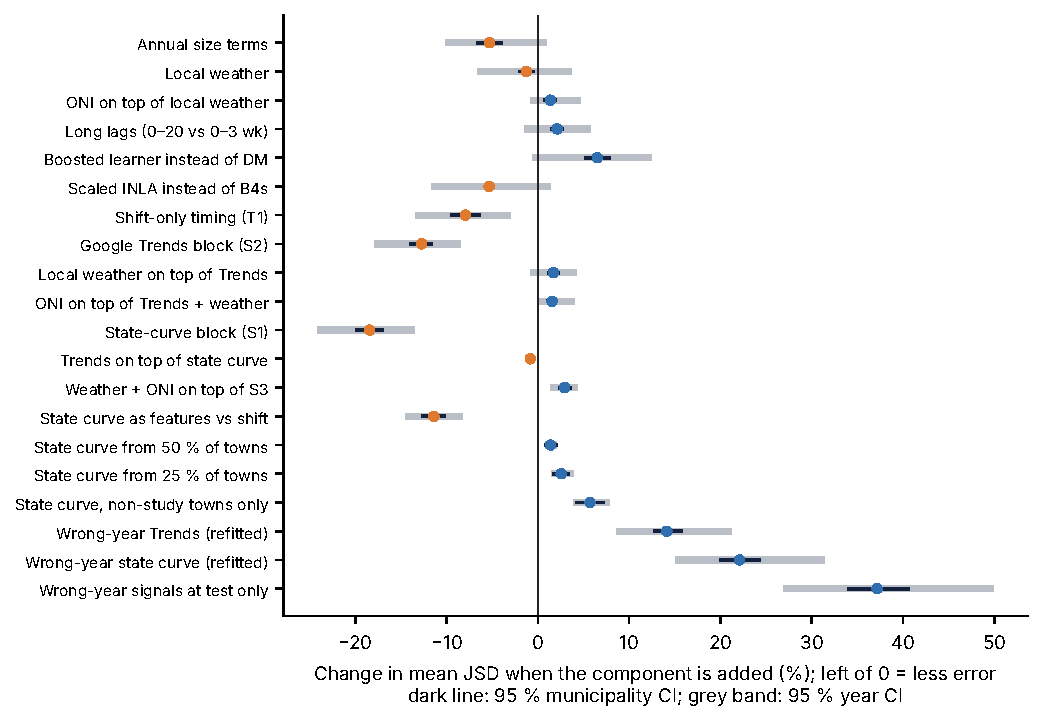
\includegraphics[width=0.92\linewidth]{figures/fig4_ablation.pdf}
\caption{Ablation forest plot: relative change in mean JSD when each component is added (dot), with 95\,\% municipality
(dark) and year (grey) bootstrap intervals.}
\label{fig:ablation}
\end{figure}

\begin{figure}[t]
\centering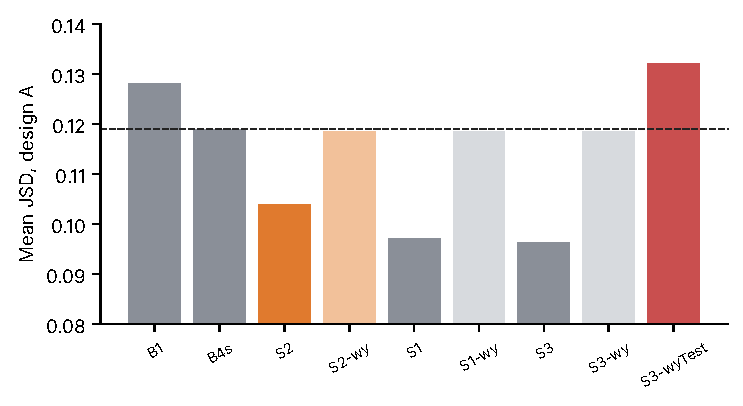
\includegraphics[width=0.7\linewidth]{figures/fig8_wrong_year.pdf}
\caption{Wrong-year controls (light bars) against the correct-year models; dashed line: B4s.}
\label{fig:wy}
\end{figure}

\section{Discussion}
\paragraph{Comparison with baselines.} The base paper's scaled INLA improves on the DM baseline by \inlaGainA\,\%, and
weather adds about 1\,\% to either model. A search signal of the same year improves the DM by \trendsGainA\,\%, more
than twice the INLA gain, with a much tighter interval across years. Weather and climate indices describe the
\emph{average} season, which the seasonal terms already capture; searches rise and fall with the year's actual epidemic
and therefore carry its timing (gap G3).

\begin{table}[t]
\centering
\small
\caption{Google Trends gain by region (design A, paired municipality bootstrap).}
\label{tab:region}
\resizebox{\linewidth}{!}{%
\begin{tabular}{lrrrrrr}
\toprule
Region & Towns & B4s & S2 (Trends) & Change \% & 95\% CI towns & Years better \\
\midrule
Center-West & 45 & 0.1276 & 0.1113 & -12.8 & [-14.3, -11.2] & 11/12 \\
North & 45 & 0.1538 & 0.1509 & -1.9 & [-3.2, -0.7] & 9/12 \\
Northeast & 45 & 0.1238 & 0.1171 & -5.4 & [-6.6, -4.4] & 10/12 \\
South & 45 & 0.1223 & 0.0949 & -22.4 & [-25.8, -19.6] & 11/12 \\
Southeast & 120 & 0.1022 & 0.0839 & -17.9 & [-19.4, -16.4] & 12/12 \\
\bottomrule
\end{tabular}}
\end{table}


\paragraph{Failure cases.} The gain is uneven (Table~\ref{tab:region}, Figure~\ref{fig:states}). It is largest in the
South and Southeast and smallest in the North (about 2\,\%). By state, Trends is worse than B4s in \statesWorse{} of
\statesTotal{} states (\statesWorseList), most of them states with very few searches before 2013, where the search
series is mostly zeros with isolated spikes and the national series is used as a fallback for empty windows. The
gain also grows with epidemic size (Table~\ref{tab:size}): in small years the search signal is weak. Figure~\ref{fig:ex}
shows typical cases, including a failure in which a late-December search spike (the start of the next season) pulls
the rebuilt curve to the end of the year.

\begin{figure}[t]
\centering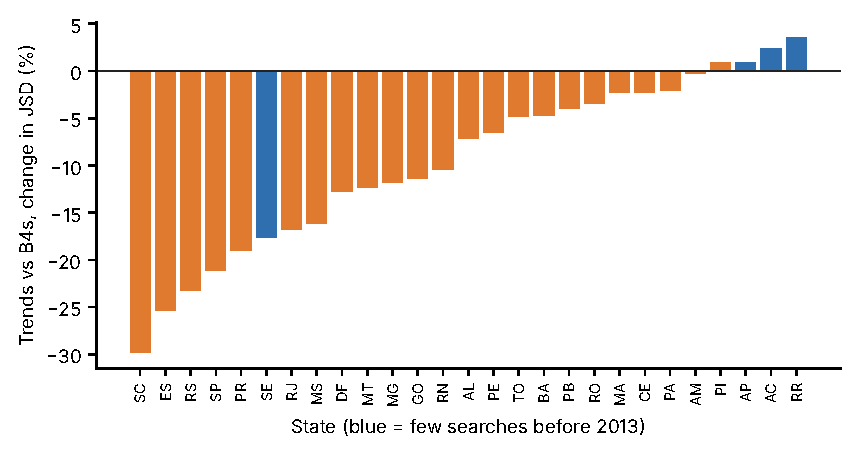
\includegraphics[width=0.92\linewidth]{figures/fig7_gain_by_state.pdf}
\caption{Trends vs B4s by state (design A), ordered by gain; blue: states with few searches before 2013.}
\label{fig:states}
\end{figure}

\begin{table}[t]
\centering
\small
\caption{Gain by epidemic size. Strata are terciles of a municipality-year's annual total divided by that municipality's median total over the test years (a descriptive split, not used by any model).}
\label{tab:size}
\resizebox{\linewidth}{!}{%
\begin{tabular}{lrrrrr}
\toprule
Year size (tercile) & n & Trends \% & CI towns & Weather \% & CI towns \\
\midrule
small year & 1065 & -8.4 & [-9.5, -7.3] & +0.5 & [-0.4, +1.5] \\
typical year & 1064 & -12.9 & [-14.5, -11.2] & -0.4 & [-1.5, +0.9] \\
large year & 1065 & -17.9 & [-19.9, -15.9] & -4.4 & [-6.0, -2.8] \\
\bottomrule
\end{tabular}}
\end{table}


\begin{figure}[t]
\centering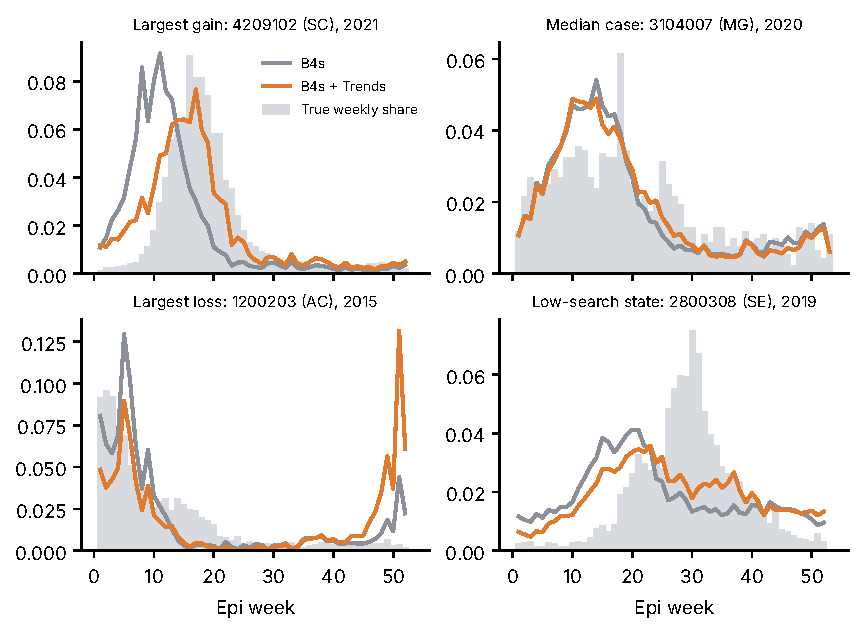
\includegraphics[width=0.92\linewidth]{figures/fig9_examples.pdf}
\caption{True weekly shares (grey) and rebuilt curves for four municipality-years selected by rule: largest gain,
median case, largest loss, and largest gain in a low-search state.}
\label{fig:ex}
\end{figure}

\paragraph{Limitations.}\label{sec:limits}
(i) The search hypotheses were formulated after the pre-registered climate results, so they are exploratory.
(ii) Google Trends starts in 2004 and is sparse in small states, which bounds where the method applies.
(iii) Scaled INLA with search data has been implemented and tested on one fold but not yet run on all folds, so the
best overall model is not yet known; INLA is also available for design A only.
(iv) Peak-week error remains about 5.8 weeks on average: timing is improved, not solved.
(v) The learning curve has at most three test years per training length, so it is descriptive (no year-level
intervals); with one or two training years the models fall back on regional profiles, and with one year the search
effect cannot be learned at all.
(vi) The state-curve models are upper bounds, valid only where neighbours report weekly in the same year.

\paragraph{Relation to the research gaps.} G1: same-year signals give each year its own shape, and the wrong-year
controls show that this is what produces the gain. G2: all results are scored against true weekly counts over 12 and 14
held-out years. G3: in the same folds, search data beat climate by an order of magnitude and make climate redundant.
G4: the ablation separates size, climate, timing shift, search and state-curve components, and the learning curve
shows how much history each component needs.

\section{Reproducibility}\label{sec:repro}
Code: \url{https://github.com/aminah9945/dengue-climate-reconstruction}, branch \texttt{results-report}. All tables,
figures and the numbers quoted in the text (\texttt{report/numbers.tex}) are written by one script that reads only the
committed result files; nothing is typed by hand.
{\footnotesize
\begin{verbatim}
pip install -e ".[all]"
# 1. data (InfoDengue, NASA POWER, ONI; about 30-45 min)
python scripts/run_pipeline.py --step data
# 2. official climate study (designs A, B, C)
python scripts/run_pipeline.py --step official --design A --climate power --subset 300
python scripts/run_pipeline.py --step official --design B --climate power --subset 300
python scripts/run_pipeline.py --step official --design C --climate power --subset 300
# 3. scaled INLA (R + R-INLA 26.8.7), design A
python -m dengue_recon.extensions.inla run --subset 300 --variants base,clim20,clim15
# 4. timing models (Google Trends snapshot in data_snapshots/google_trends)
export TIMING_TRENDS_DIR=$PWD/data_snapshots/google_trends
python -m dengue_recon.extensions.timing.run --design A --subset 300
python -m dengue_recon.extensions.timing.run --design C --subset 300
python -m dengue_recon.extensions.timing.run --design A --models B4s,M1-noONI,S2,S2C,S2C-noONI \
       --out results/extensions/timing/runs_s2c
python -m dengue_recon.extensions.timing.run --design C --models B4s,M1-noONI,S2,S2C,S2C-noONI \
       --out results/extensions/timing/runs_s2c
# 4b. learning curve with search data (design B, k = 2..13; and k = 1: train 2010, test 2011)
python -m dengue_recon.extensions.timing.run --design B --out results/extensions/timing/runs_lc
python -m dengue_recon.extensions.timing.run --design A --years 2011 \
       --models B1,B4s,M1-noONI,S2,S2C-noONI --out results/extensions/timing/runs_lc
# 5. every table, figure and number of this report
python scripts/make_results_report.py
\end{verbatim}
}
Colab notebooks \texttt{notebooks/06\_official\_experiments.ipynb}, \texttt{07\_timing\_model.ipynb} and
\texttt{08\_google\_trends\_download.ipynb} run the same steps. Run logs, per-fold checkpoints and check files are under
\texttt{results/}.

\end{document}
